\label{chap:validation}

\section{Why the Graph Needs Independent Validation}
\label{sec:val-why}

There is no ground truth for causal links in the real atmosphere, and PCMCI's guarantees rest on assumptions that hold only approximately. Stage~B therefore applies four checks in a fixed order, each of which can \emph{reject} links even though none can prove a link correct (Figure~\ref{fig:validation}). The resulting graph is frozen before any test year is used.

\begin{figure}[htbp]
\centering
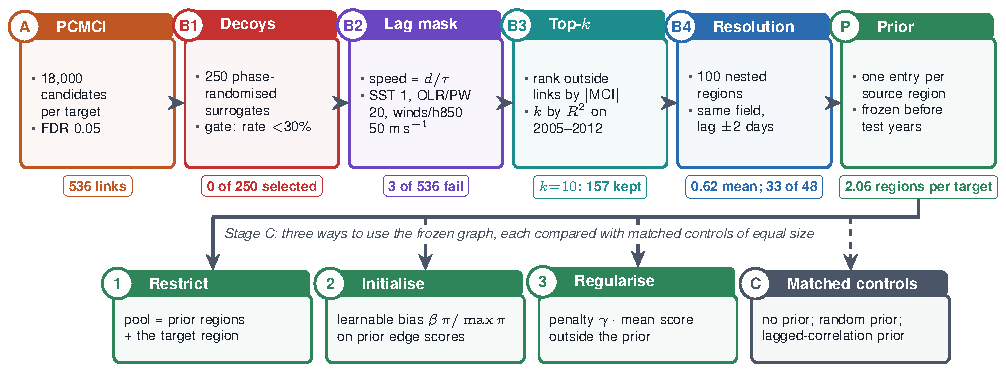
\includegraphics[width=\textwidth]{workflows/wf_validation.pdf}
\caption{Stage~B validation and Stage~C use of the graph. The tags under each check give the measured outcome (Chapter~\ref{chap:results}). The frozen region-level prior enters the splitter in one of three modes and is compared with matched controls of equal size.}
\label{fig:validation}
\end{figure}

\section{B1: Surrogate Decoys}
\label{sec:val-b1}

The first check asks whether the pipeline selects series merely because they have realistic memory. Decoys are phase-randomised copies of real nodes~\cite{theiler1992testing,schreiber2000surrogate}. A series $x_t$ is Fourier-transformed, its phases are replaced by independent uniform random phases, and it is transformed back:
\begin{equation}
  \tilde{x}_t=\frac{1}{n}\sum_f |\hat{x}_f|\,e^{i\theta_f}\,e^{2\pi i f t/n},\qquad \theta_f\sim\mathcal{U}[0,2\pi).
  \label{eq:phaserand}
\end{equation}
The decoy keeps the power spectrum, and therefore the autocorrelation including the 30--60-day BSISO peak, but has no real relationship with any node. 250 decoys are added to the 300 real nodes in a separate PCMCI pass (550 nodes, 33{,}000 candidates per target). The \emph{decoy rate} $\delta$ is the fraction of decoys selected as a parent of any target, and the pre-set warning line is $\delta\ge30\%$. Decoys do not reproduce non-Gaussian amplitudes, seasonal changes in variance, or a common driver shared with the target, so a low decoy rate rules out autocorrelation-driven selection but does not by itself prove causality.

\section{B2: Physical Lag Mask}
\label{sec:val-b2}

A link from region $r'$ to region $r$ at lag $\tau$ requires a signal to travel at least the closest great-circle distance $d(r',r)$ between the two regions in $\tau$ days. Its implied speed is
\begin{equation}
  s_e=\frac{d(r',r)}{\tau\times 86{,}400\,\mathrm{s}},
  \label{eq:speed}
\end{equation}
and the link fails if $s_e$ exceeds a generous limit for its source field: 1\ms\ for SST, whose own influence is ocean-mediated; 20\ms\ for OLR and PW, the upper range of convectively coupled Kelvin waves~\cite{kiladis2009convectively}; and 50\ms\ for the wind and height fields, which can be carried by fast equatorial waves. Unlike a distance cutoff, this test keeps remote teleconnections that act at plausible speeds. Links at lags of 25 days or more are flagged as possible echoes of the 30--60-day oscillation. Failing links are removed from the forecasting prior but kept, with their flags, in the graph file for inspection.

\section{B3: Data-Driven Top-\texorpdfstring{$k$}{k}}
\label{sec:val-b3}

Each target's outside links, those from other regions, are ranked by $|\hat\rho^{\,\mathrm{MCI}}|$. For each $k=0,\dots,10$, a ridge regression on the target's own-region links plus its top-$k$ outside links is fitted on 1979--2004 season days and scored by $R^2$ on 2005--2012; $k$ is chosen as the maximiser. The test period plays no part. The step sets the size of the prior from data and caps the number of drivers per target.

\section{B4: Resolution Persistence}
\label{sec:val-b4}

A link that is an artefact of how the regions were drawn should be fragile under a different partition. Stage~A is rerun at 100 nested regions (each region split in two). An outside link persists if some child pair carries a link from the same field at a lag within $\pm2$ days. The persistence score of target $r$ is the fraction of its outside links that persist, and a target passes if $\Pi_r\ge0.5$. Failures are flagged rather than deleted, because a real large-scale signal can be diluted at a finer scale.

\section{From Validated Links to a Region-Level Prior}
\label{sec:moe-prior}

The splitter chooses whole source regions, and the field chosen within a region is the least stable part of the graph. Validated outside links are therefore merged per source region:
\begin{equation}
  \pi_r(r')=\max_{e:\ \mathrm{src}(e)=r'}\ |\hat\rho^{\,\mathrm{MCI}}_e|,
  \label{eq:prior}
\end{equation}
over the links that pass B1 and B2 and survive B3. Field and lag details remain in the frozen graph file.

\section{The Graph-Guided Mixture of Experts}
\label{sec:moe-arch}

Each region has its own causal splitter and expert, 50 independent pairs trained from scratch with no weight sharing. Over time each region keeps a lineage of experts managed by the lifecycle of Section~\ref{sec:lifecycle}, which makes the system a Mixture of Experts in which a region's active expert can change with the regime~\cite{jacobs1991adaptive}.

\paragraph{Candidate pools.} The splitter of target $r$ considers either its adjacent regions (\emph{direct}, about 6--8), neighbours of neighbours (\emph{2hop}, about 15--23), or all 50 regions (\emph{full}). The target region is always a candidate.

\label{sec:moe-splitter}
\paragraph{Causal splitter.} Following DIR~\cite{wu2022discovering}, a rationale generator scores each candidate edge from a 10-day window of the two regions' histories,
\begin{equation}
  a_{r'r,t}=\sigma\big(\mathrm{MLP}[\mathbf{w}^{r'}_t\,\|\,\mathbf{w}^{r}_t]+b_{r'r}\big),
  \label{eq:score}
\end{equation}
where $b_{r'r}$ is an optional prior bias. The top fraction $\min(0.5,3/|\mathcal{C}_r|)$ of edges forms the causal set; the remaining edges are swapped with the same edges on $M=6$ other days to create interventions. The splitter minimises the mean and variance of the risk across interventions,
\begin{equation}
  \mathcal{L}_{\mathrm{split}}=\frac{1}{M}\sum_{m}\ell_{t,m}+\lambda\,\mathrm{Var}_m[\ell_{t,m}],
  \label{eq:dirloss}
\end{equation}
with $\lambda$ warmed up from 0 to 1. A spurious head with detached gradients serves as a leakage check.

\paragraph{Expert.} The expert aggregates the selected sources' 49-value feature vectors, weighted by their splitter scores, and maps the result to the forecast with a small MLP. The target's own history enters only if the target region is selected, so the forecast depends on the splitter's choice. A splitter is \emph{informative} if the spread of its candidates' mean scores is $\sigma_a\ge0.02$; below that the scores cluster around one value and the selection is effectively random.

\section{Three Ways to Use the Graph}
\label{sec:moe-modes}

\begin{itemize}
  \item \textbf{Restrict:} the candidate pool becomes the prior regions plus the target, $\mathcal{C}_r=\{r'\in\pi_r\}\cup\{r\}$.
  \item \textbf{Initialise:} the pool is unchanged, and the learnable bias in Eq.~\eqref{eq:score} starts at $b_{r'r}=2\,\pi_r(r')/\max\pi_r$ for prior regions and 0 otherwise.
  \item \textbf{Regularise:} the pool is unchanged, and a penalty $\gamma\cdot\mathrm{mean}(a_{r'r})$ over candidates outside the prior is added to the loss.
\end{itemize}
To attribute an effect to the graph's content, each mode is compared with matched controls of equal size per target: no prior, a random prior (the same number of regions drawn at random with the strengths shuffled), and a lagged-correlation prior (the regions most correlated with the target on training data).

A link at lag $\tau$ can inform a direct forecast at lead $L$ only if $\tau\ge L$, because the source value it describes must be known at the issue time. A graph whose links act within one or two days is therefore matched to short-lead forecasts.

\section{Drift Detection and the Expert Lifecycle}
\label{sec:lifecycle}

Figure~\ref{fig:lifecycle} shows how each region's expert is kept current.

\begin{figure}[htbp]
\centering
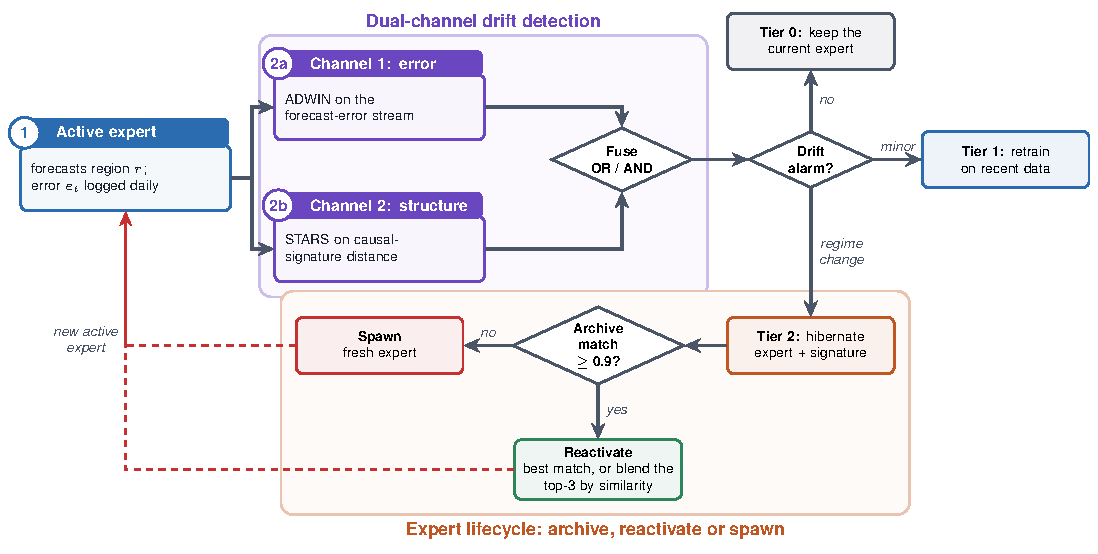
\includegraphics[width=\textwidth]{workflows/wf_lifecycle.pdf}
\caption{Drift detection and the expert lifecycle for one region. Two channels watch the forecast error and the causal structure; a fused alarm leads to retraining, or to archiving the expert and then reactivating a matching archived expert or spawning a fresh one.}
\label{fig:lifecycle}
\end{figure}

\paragraph{Channel 1: error (ADWIN).} ADWIN~\cite{bifet2007learning} keeps an adaptive window of recent forecast errors. Whenever two sub-windows have significantly different mean errors, it drops the older part and raises an alarm. For a window $W$ split into sub-windows $W_0$ and $W_1$ with means $\hat\mu_0,\hat\mu_1$ and sizes $n_0,n_1$, a change is declared if
\begin{equation}
  |\hat\mu_0-\hat\mu_1|>\epsilon_{\mathrm{cut}}=\sqrt{\frac{1}{2m}\ln\frac{4|W|}{\delta}},\qquad m=\Big(\frac{1}{n_0}+\frac{1}{n_1}\Big)^{-1},
\end{equation}
where $\delta$ is the confidence parameter.

\paragraph{Channel 2: causal structure (STARS).} The splitter's per-edge score vector on each day is the region's causal signature; its cosine distance from a reference signature (the mean over a baseline window) forms a scalar causal-structure series. Rodionov's STARS test~\cite{rodionov2004sequential} flags a point that falls outside the current regime's range and confirms a shift only if the following $\ell$ points support the new level. For a candidate shift at time $j$, the regime-shift index
\begin{equation}
  \mathrm{RSI}_j=\sum_{i=j}^{j+m}\frac{x_i-\bar{x}_{\mathrm{crit}}}{\ell\,\hat\sigma_\ell},\qquad m=0,\dots,\ell-1,
\end{equation}
must keep its sign over the cut-off length $\ell$, where $\bar{x}_{\mathrm{crit}}$ is the level that a new regime's mean must exceed at the chosen significance and $\hat\sigma_\ell$ is the average standard deviation over intervals of length $\ell$. Because it watches the structure rather than the outcome, it can in principle detect a change before forecasts degrade.

\paragraph{Fusion.} The channels are combined with OR, which reacts faster but raises more alarms, or with AND, which is slower but has fewer false alarms.

\paragraph{Lifecycle.} After an alarm, a minor change triggers retraining (Tier~1). A regime change (Tier~2) hibernates the current expert together with its causal signature and searches the archive. If an archived expert's signature has cosine similarity of at least 0.9, it is reactivated, either the single best match or a similarity-weighted blend of the three best matches; otherwise a fresh expert is spawned. Because climate regimes such as ENSO phases recur, reactivation reuses knowledge instead of relearning it, and adding experts rather than overwriting them limits catastrophic forgetting~\cite{kirkpatrick2017overcoming}.

\paragraph{Stage D: structural drift of the PCMCI graph.} Separately, PCMCI is rerun on sliding windows of one or three BSISO seasons, restricted to each target's B1/B2-validated candidates. The distance $\Delta_w=1-J(\mathcal{P}_w,\mathcal{P}_{w-1})$ between consecutive parent sets, where $J$ is the Jaccard similarity, is tested with STARS and compared with ENSO phase changes derived from the project's own SST.

\section{Consolidated Algorithm}
\label{sec:moe-algorithm}

Algorithm~\ref{alg:build-validate} summarises Phase~1. Every step before the freeze uses 1979--2012 only.

\begin{algorithm}[htbp]
\caption{Build, validate, freeze and use the causal graph, and keep experts current}
\label{alg:build-validate}
\small
\begin{algorithmic}[1]
\State compute the BSISO index and season $\mathcal{S}$ (EOF fitted on 1979--2012)
\State \textbf{Stage A:} run PCMCI (Algorithm~\ref{alg:pcmci}) for each of the 50 OLR targets
\State \textbf{B1:} add 250 phase-randomised decoys in a separate pass; stop if the decoy rate is $\ge 30\%$
\State \textbf{B2:} compute implied speeds; remove links above the field's limit from the prior
\State \textbf{B3:} choose $k$ by validation $R^2$; keep the top-$k$ outside links per target
\State \textbf{B4:} rerun PCMCI at 100 regions; flag targets with $\Pi_r<0.5$
\State build the region prior $\pi_r$ (Eq.~\ref{eq:prior}) and \textbf{freeze} graph and prior
\State \textbf{Stage C:} train a splitter and expert per region with the prior (restrict, initialise or regularise) and with matched controls; score on 2013--2022
\For{each day in the monitored period} \Comment{lifecycle}
  \State update ADWIN (error) and STARS (structure); fuse with OR or AND
  \If{alarm} retrain, or hibernate and reactivate a matching archived expert (similarity $\ge 0.9$), or spawn
  \EndIf
\EndFor
\State \textbf{Stage D:} sliding-window PCMCI, $\Delta_w$, STARS and comparison with ENSO
\end{algorithmic}
\end{algorithm}
